\documentclass[border=4pt]{standalone}
\usepackage{tikz}
\usepackage{xcolor}
\usetikzlibrary{arrows.meta, positioning}
\newcommand{\pillar}[1]{\textcolor{blue!55!black}{\footnotesize\itshape #1}}
\begin{document}
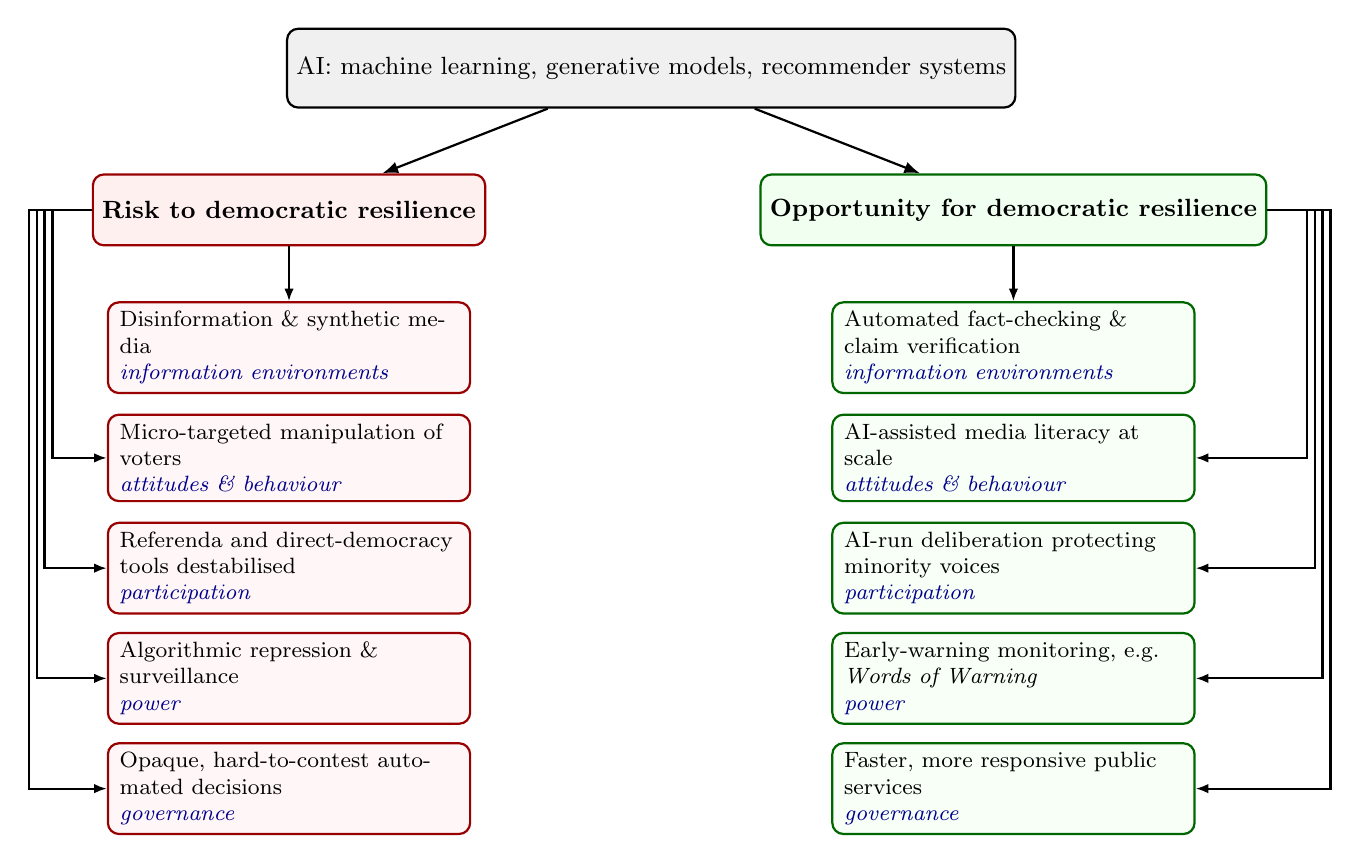
\begin{tikzpicture}[
  every node/.style = {font=\small},
  root/.style = {draw, rounded corners, fill=gray!12, align=center, minimum width=4.6cm, minimum height=1cm},
  branch/.style = {draw, rounded corners, align=center, minimum width=4.6cm, minimum height=0.9cm, font=\bfseries\small},
  leaf/.style = {draw, rounded corners, align=left, minimum width=4.6cm, text width=4.3cm, minimum height=1.05cm, font=\footnotesize},
  pillar/.style = {font=\scriptsize\itshape},
  >=Latex, thick
]
  \node[root] (ai) at (0,4.1) {AI: machine learning, generative models, recommender systems};

  \node[branch, draw=red!60!black, fill=red!6] (risk) at (-4.6,2.3) {Risk to democratic resilience};
  \node[branch, draw=green!40!black, fill=green!6] (opp) at (4.6,2.3) {Opportunity for democratic resilience};

  \draw[-{Latex[length=2mm]}] (ai) -- (risk);
  \draw[-{Latex[length=2mm]}] (ai) -- (opp);

  \node[leaf, draw=red!60!black, fill=red!3] (r1) at (-4.6,0.55) {Disinformation \& synthetic media\\\pillar{information environments}};
  \node[leaf, draw=red!60!black, fill=red!3] (r2) at (-4.6,-0.85) {Micro-targeted manipulation of voters\\\pillar{attitudes \& behaviour}};
  \node[leaf, draw=red!60!black, fill=red!3] (r3) at (-4.6,-2.25) {Referenda and direct-democracy tools destabilised\\\pillar{participation}};
  \node[leaf, draw=red!60!black, fill=red!3] (r4) at (-4.6,-3.65) {Algorithmic repression \& surveillance\\\pillar{power}};
  \node[leaf, draw=red!60!black, fill=red!3] (r5) at (-4.6,-5.05) {Opaque, hard-to-contest automated decisions\\\pillar{governance}};

  \node[leaf, draw=green!40!black, fill=green!3] (o1) at (4.6,0.55) {Automated fact-checking \& claim verification\\\pillar{information environments}};
  \node[leaf, draw=green!40!black, fill=green!3] (o2) at (4.6,-0.85) {AI-assisted media literacy at scale\\\pillar{attitudes \& behaviour}};
  \node[leaf, draw=green!40!black, fill=green!3] (o3) at (4.6,-2.25) {AI-run deliberation protecting minority voices\\\pillar{participation}};
  \node[leaf, draw=green!40!black, fill=green!3] (o4) at (4.6,-3.65) {Early-warning monitoring, e.g.\ \emph{Words of Warning}\\\pillar{power}};
  \node[leaf, draw=green!40!black, fill=green!3] (o5) at (4.6,-5.05) {Faster, more responsive public services\\\pillar{governance}};

  \draw[-{Latex[length=1.6mm]}] (risk.south) -- (r1.north);
  \draw[-{Latex[length=1.6mm]}] (risk.west) -- ++(-0.5,0) |- (r2.west);
  \draw[-{Latex[length=1.6mm]}] (risk.west) -- ++(-0.6,0) |- (r3.west);
  \draw[-{Latex[length=1.6mm]}] (risk.west) -- ++(-0.7,0) |- (r4.west);
  \draw[-{Latex[length=1.6mm]}] (risk.west) -- ++(-0.8,0) |- (r5.west);
  \draw[-{Latex[length=1.6mm]}] (opp.south) -- (o1.north);
  \draw[-{Latex[length=1.6mm]}] (opp.east) -- ++(0.5,0) |- (o2.east);
  \draw[-{Latex[length=1.6mm]}] (opp.east) -- ++(0.6,0) |- (o3.east);
  \draw[-{Latex[length=1.6mm]}] (opp.east) -- ++(0.7,0) |- (o4.east);
  \draw[-{Latex[length=1.6mm]}] (opp.east) -- ++(0.8,0) |- (o5.east);
\end{tikzpicture}
\end{document}
